\documentclass{article}
\usepackage{graphicx}
\usepackage{fullpage}
\usepackage{float}
\title{Implementation and comparrison exponential function algoritms}
\author{Andreas}
\date{}
\begin{document}
\maketitle

\section{Algoritms}
The expotential function, defined by the sum. ~\cite{expref}
	\begin{equation}\label{eq:exp}
\exp (x) := \sum_{k = 0}^{\infty} \frac{x^k}{k!} = 1 + x + \frac{x^2}{2} + \frac{x^3}{6} + \frac{x^4}{24} + \cdots\;.
	\end{equation}
A numerical approximation of this function is found using the c built-in math.h related libary.
Another numerical approximation of this function is presented in ~(\ref{eq:approx1}) 
	\begin{equation}\label{eq:approx1}
\exp (x) := 1 + x(1+\frac{x}{2}(1+\frac{x}{3}(1+\frac{x}{4}(1+\frac{x}{5}*(1+\frac{x}{6}(1+\frac{x}{7}(1+\frac{x}{8}(1+\frac{x}{9}(1+\frac{x}{10})))))))))\;.
	\end{equation}
By examination it is clear that this is the expanded formula of the function in ~(\ref{eq:exp}):
	\begin{equation}\label{eq:deri1}
\exp (x) := 1 + (x+\frac{x^2}{2}(1+\frac{x}{3}(1+\frac{x}{4}(1+\frac{x}{5}*(1+\frac{x}{6}(1+\frac{x}{7}(1+\frac{x}{8}(1+\frac{x}{9}(1+\frac{x}{10}))))))))\;.
	\end{equation}
	\begin{equation}\label{eq:deri2}
\exp (x) := 1 + (x+\frac{x^2}{2}+\frac{x^3}{6}(1+\frac{x}{4}(1+\frac{x}{5}*(1+\frac{x}{6}(1+\frac{x}{7}(1+\frac{x}{8}(1+\frac{x}{9}(1+\frac{x}{10})))))))\;.
	\end{equation}
And so on, until the equation becomes 
	\begin{equation}\label{eq:deri2}
\exp (x) := 1 + (x+\frac{x^2}{2}+\frac{x^3}{6}(1+...\frac{x^{10}}{3628800})))))))))\;.
	\end{equation}
For small x, it is reasonable that this function is a good approximation as $x^{10}$ is much smaller than !10.
In the algorithm this is explotied with the statement if(x>1./8)return pow(exp(x/2),2). This ensures that the function
is calculated precisely even as x becomes large.

The algorithm is plotted from x=0-5 in figure along with the algorithm from math.h. 
\section{Figures}
	\begin{figure}[H]\centering \label{fig:exponential function}
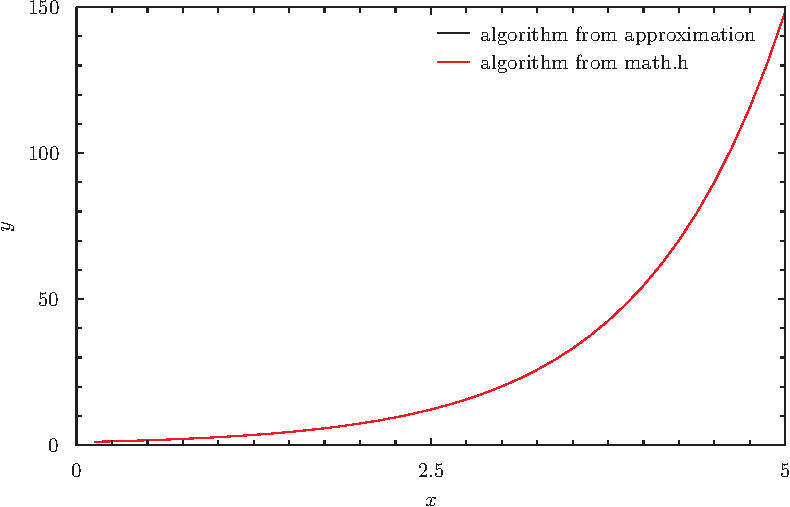
\includegraphics{fig-exp-pyxplot.pdf}
\caption{empty}
	\end{figure}
There is clear overlap between the two algorithms, and they must be nealy identical.

\begin{thebibliography}{9}
\bibitem{expref} Eric W. "Exponential Function". mathworld.wolfram.com. Retrieved 2020-08-28
\end{thebibliography}

\end{document}

